\documentclass[11pt]{article}
\usepackage{fullpage}
\usepackage[utf8]{inputenc}
\usepackage{algorithm}
\usepackage[noend]{algpseudocode}
\usepackage{hyperref}
\usepackage{amssymb}
\usepackage{amsmath}
\usepackage{amsthm}
\usepackage{graphicx}
\usepackage{cite}
\usepackage{appendix}
\newtheorem{theorem}{Theorem}
\newtheorem{proposition}{Proposition}
\newtheorem{lemma}{Lemma}
\theoremstyle{definition} 
\newtheorem{definition}{Definition}
\newtheorem{claim}{Claim}
\newtheorem{corollary}{Corollary}
\newtheorem{observation}{Observation}

\hypersetup{
  colorlinks   = true,    % Colours links instead of ugly boxes
  urlcolor     = blue,    % Colour for external hyperlinks
  linkcolor    = blue,    % Colour of internal links
  citecolor    = red      % Colour of citations
}

\title{Auditable and Access-Control Objects: A Comparative Analysis of Synchronization and Consensus}
\author{Tal Zohar, Adi Rivkin}
\date{\today}

\begin{document}
    \maketitle

\section{Introduction}	
In the field of distributed systems, synchronization and auditability play pivotal roles in the design and analysis of robust systems. 
This article aims to investigate two recently proposed and seemingly unrelated objects in this field. We will compare and contrast the distributed implementation of these objects and their synchronization characteristics within Herlihy’s consensus hierarchy \cite{herlihy1991wait}. 

The first object is an \textit{auditable register} first introduced by \cite{cogo_et_al:LIPIcs.DISC.2021.53} and further examined in \cite{AuditableRegs}. This register extends traditional R/W registers to include an audit operator that lists all prior performed read operations.
On the other hand, \cite{AccessControl} recently introduced the notion of \textit{Access-Control} objects which govern access to some resource. It examines the synchronization characteristics of two objects: \textit{AllowList} and \textit{DenyList}.

In this article we will show that even though the aforementioned objects have very different use-cases, they are structurally similar. This similarity gives way to perform comparison between the two. We will show how the insights and methodologies from each paper complement each other, leading to new results and a deeper understanding of the synchronization required for the objects. 

The structural parallels are apparent when we consider that both object types support three operation types, where each can be applied by a specific class of processes. Moreover, we can give each of the three operations some general title that holds in both object types.
\begin{enumerate}
    \item An operation that outputs the "access" history of the register. Essentially, this operation supports the concept of \textit{auditablility}.
    \item An operation that performs some "access" to the register. This operation is tracked in the "access" history.
    \item An operation that fundamentally changes the inner state of the register. This operation is not necessarily tracked in the "access" history.
\end{enumerate}

\textbf{Organization of the paper.} In section 2 we provide some basic definitions and define the two aforementioned object types. Additionally, we provide some new definitions that we believe better encapsulate the differences and similarities between the two objects. Namely, we define the object of \textit{AAL} that gives an alternative definition for \textit{AllowList}. Additionally, we define \textit{ADL} and \textit{HADL} that provide different alternative definitions for \textit{DenyList}. Lastly we define object \textit{HAA} as a spin on \textit{AtomicAudit}. In section 3 we provide consensus number lower-bounds on our newly-defined objects, as well as strengthen some lower-bounds of some previously-established objects. Finally sections 4,5 provide consensus number upper-bounds on our newly-defined objects, as well as strengthen some upper-bounds of some previously-established objects.

\section{Old  and New Definitions}
\subsection{Standard Definitions}
In the following article we will use some standard definitions in the field of synchronicity. 

We operate in the model of crash-prone asynchronous processes with communication via shared memory.

Given an execution of an algorithm, we define its \textit{history} to be the sequence of invocations and responses given by the execution. An invocation that lacks a corresponding response is referred to as a \textit{pending invocation}. A \textit{sequential history} is a history where each invocation is immediately followed by a response - making all operations seem atomic. We define $complete(H)$ to be set the of histories derived from $H$ by adding responses to some of the pending invocations and removing the rest.

The consensus number of an object of type $T$ represents the maximum number of processes for which it is possible to implement a wait-free consensus object using only atomic R/W registers and objects of type $T$.

A Single Writer Multi-Reader \textit{Atomic Snapshot} object \cite{afek1993atomic} is a fixed-size array that supports two operations: \textit{Snapshot} and \textit{Update}. The \textit{Snapshot}() operation lets a process atomically read the entire array, while the  \textit{Update}($v, i$) operation allows $p_i$ to write $v$ to the $i$'th array position. \cite{afek1993atomic} showed that the object can be implemented the object in a wait-free manner using only R/W registers.

Finally, define the \textit{Swap} and \textit{Fetch\&add} operations on some register $R$ as follows: A \textit{Swap}(v) operation atomically replaces the register’s value with $v$ and returns the original value. A \textit{Fetch\&add}($a$) operation atomically updates the register by adding $a$ to its current value and returns the original value.

\subsection{Object Definitions}

In the following section we will provide definitions for all the relevant objects of the article. We will redefine the objects of \cite{AccessControl, AuditableRegs} (slightly changing their formulations for consistency sake), and by doing so we hope that the structural similarities of the objects will be apparent. 

In addition to that, we will define some new alternative definitions for these objects which will help us perform the comparison. As we will see, some of our new alternative definitions will be equivalent to their original counterparts and some will be inherently different.


The following two definitions are taken from \cite{AuditableRegs}. These two definition provide different specifications for an \textit{Auditable} register, which is essentially a R/W register that supports also an \textit{Audit} operation that returns all values read from the register along with the identity of the readers.

\begin{definition}
The $AtomicAudit$ object supports the following operations: \mbox{WRITE}, \mbox{READ}, \mbox{AUDIT}. Given history $H$ there exists $H'\in \mbox{complete}(H)$ and a sequential history $\pi$ such that:
\begin{itemize}
\item \textit{Linearizability}. If operation $op_1$ precedes operation $op_2$ in $H$ then $op_1$ appears before $op_2$ in $\pi$.
  \item \textit{Termination}. All operations must return when called by a correct process.
  \item \textit{\mbox{READ} Validity}. The invocation of \mbox{READ} will return value of the most recent preceding WRITE operation in $\pi$.
  \item \textit{\mbox{AUDIT} Validity}.  The invocation of \mbox{AUDIT} by process $p$ returns a set of pairs $\mathcal{P}$ that satisfy:
  \begin{itemize}
  \item \textit{Completeness}. For each read operation $op$ that precedes the audit in $\pi$, then $(p,v)\in \mathcal{P}$ where $p$ is the process that invokes $op$ and $v$ is the return value of $op$.
  \item \textit{Strong Accuracy}. For each $(p,v)\in \mathcal{P}$ there exists a read operation invoked by $p$ that returns $v$ and additionally precedes the audit in $\pi$.

\end{itemize}

\end{itemize}

\end{definition}


\begin{definition}
The $RegularAudit$ object is defined like $AtomicAudit$ with the exception of the following \textit{\mbox{AUDIT} Validity} relaxation:
\begin{itemize}
  \item \textit{\mbox{AUDIT} Validity}.  The invocation of \mbox{AUDIT} by process $p$ returns a set of pairs $\mathcal{P}$ that satisfy:
  \begin{itemize}
  \item \textit{Weak-Completeness}. For each read operation $op$ in $H'$ that completes before the invocation of the audit in $H'$, we have $(p,v)\in \mathcal{P}$ where $p$ is the process that invokes $op$ and $v$ is the return value of $op$.
  \item \textit{Strong Accuracy}. For each $(p,v)\in \mathcal{P}$ there exists a read operation invoked by $p$ that returns $v$ and that its invocation precedes the audit's completion in $H'$.

\end{itemize}

\end{itemize}

\end{definition}

Informally, $RegularAudit$ relaxes the \textit{\mbox{AUDIT} Validity} property to be defined over the non overlapping operations of $H'$ instead of the sequential history $\pi$.

On the other hand, \cite{AccessControl} defines the $AllowList$ and $DenyList$ objects. These objects allows a set of managers to govern access to some resource. In this scenario, processes which want access to some resource must prove that they are authorized for it. The $AllowList$ and $DenyList$ objects provide implementations for two interpretation of this scenario. 

The $AllowList$ object provides authorization using a whitelist. The managers can add elements to the whitelist. In order to receive access to the resource a process must prove that it knows some element previously authorized by a manager.

Formally, we divide all processes  $\Pi$ into three groups. The provers denoted by $\Pi_V \subseteq \Pi$ are the processes that can invoke a $\mbox{PROVE}(v)$ operation in order to gain access to some resource. This proof is valid if at the time of its invocation $v$ was whitelisted. A value $v$ can be whitelisted by a manager process using an $\mbox{APPEND}(v)$ operation. The predefined set $\mathcal{S}$ denotes all possible whitelistable values. We denote all managers by $\Pi_M\subseteq \Pi$. Finally, all auditor processes denoted by $\Pi_A\in \Pi$ can perform a $\mbox{PROOF-AUDIT}()$ operation to receive all valid proofs invoked until that point, together with the process id of the prover. 

Note that we slightly altered the original formulation which assumes that all processes are permitted to invoke $\mbox{PROOF-AUDIT}()$. We will later show how this specification allows us to achieve tighter consensus number bounds.

\begin{definition}
The $AllowList$ object ($AL$ in short) supports the following operations: \mbox{APPEND}, \mbox{PROVE}, \mbox{PROOF-AUDIT}. Given history $H$ there exists $H'\in \mbox{complete}(H)$ and a sequential history $\pi$ such that:
\begin{itemize}
\item \textit{Linearizability} and \textit{Termination}. Same as before.
  \item \textit{\mbox{APPEND} Validity}. The invocation of \mbox{APPEND} by process $p$ is valid iff. $p\in \Pi_M$ and $v \in \mathcal{S}$.
  \item \textit{PROOF-AUDIT Validity}. Every PROOF-AUDIT operation returns a list of all valid proofs (alongside their prover's id) that appear before it in $\pi$.
  \item \textit{Optional - Anonymity}. If process $p$ invokes a READ() operation, it gains no information of the proven values $v$.
  \item \textit{\mbox{PROVE} Validity}.
  \begin{itemize}
   \item \textit{Correctness}.  If the invocation of \mbox{PROVE}(v) by process $p$ is valid then $p\in \Pi_V$ and there exists a preceding APPEND(v) operation in $\pi$.
  \item \textit{Progress}. If a valid APPEND(v) is invoked then there exists a point in $\pi$ such that any PROVE(v) invoked after this point by any process $p\in \Pi_V$ will be valid.
  \end{itemize}
\end{itemize}

\end{definition}

The definition above is taken from \cite{AccessControl} and slightly modified for readability. We now move on to suggest an alternative definition for AllowList. 

\begin{definition}\label{def:AAL}[\textit{Alternative-AllowList} definition, \textit{AAL} in short]
We alter the \textit{\mbox{PROVE} Validity} property as follows:
\begin{itemize}
   \item \textit{Weak-Completeness}. If there exists a valid \mbox{APPEND}(v) operation in $H'$ that completes before the invocation of a \mbox{PROVE}(v) operation in $H'$ by some $p\in \Pi_V$ then the prove operation is valid. 
  \item \textit{Weak-Accuracy}. If the invocation of PROVE(v) is valid by process $p$, then $p \in \Pi_V$ and there exists a valid \mbox{APPEND}(v) operation that is invoked in $H'$ 
 before the completion of the prove operation.
\end{itemize}
\end{definition}

\begin{figure}
    \centering
    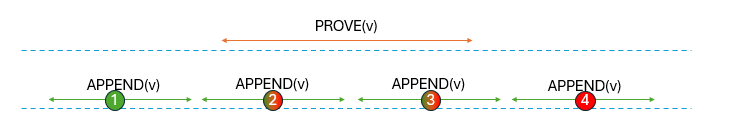
\includegraphics[width=1\linewidth]{Relaxation.png}
    \caption{Illustration for the alternative \textit{\mbox{PROVE} Validity} definition for \textit{AAL}. The illustration exhibits a PROVE(v) operation alongside four different options for an APPEND(v) operation. In the first option, the APPEND \textbf{must} be noticed by the PROVE. In the second and third options, the APPEND \textbf{can} be noticed by the PROVE. In the fourth option, the APPEND has no influence on the PROVE.}
    \label{fig:enter-label}
\end{figure}


Definition~\ref{def:AAL} takes inspiration from the definition of \textit{RegularAudit}. However, note that while \textit{RegularAudit} performs a relaxation of the \textit{Audit} property, in our case \textit{AAL} suggests a relaxation of the \textit{Prove} property. We believe that Definition~\ref{def:AAL} gives a more robust and comprehensive definition for the object of \textit{AllowList}. The following theorem provides justification for shifting our focus to this alternative definition.


\begin{theorem}\label{thm:AALEquivelancy}
    Every object implementation of \textit{Alternative-AllowList} implements also \textit{AllowList}.
\end{theorem}


The proof of Theorem~\ref{thm:AALEquivelancy} is located at Appendix~\ref{prf:AALEquivelancy}. In other words we will say that \textit{AAL} is \textbf{stronger} than \textit{AL}. With that in mind, we claim that they are equivalent in terms of their required synchronicity. Obviously, a lower bound for the consensus number of \textit{AL} implies a lower bound for the consensus number of \textit{AAL}. Although the converse is not necessarily true, we note that the upper bound for \textit{AL} provided in \cite{AccessControl} can be directly applied on \textit{AAL}. More specifically, \cite{AccessControl} provides an implementation of \textit{AL} using R/W objects (and other object of consensus number 1). The aforementioned implementation satisfies all properties of \textit{AAL} and therefore \textit{AAL} has consensus number 1.

\vspace{1em}

On the other hand, the $DenyList$ object provides authorization using a blacklist. The managers can revoke users by adding elements to the blacklist. In order to receive access to the resource a process must prove that it knows some element that wasn't previously revoked by a manager.

\begin{definition}
The $DenyList$ object ($DL$ in short) is defined like $AllowList$ with the following alternate \textit{\mbox{PROVE} Validity} definition:
\begin{itemize}
   \item \textit{Strong-Accuracy}. If the invocation of \mbox{PROVE}(v) by process $p$ is invalid then either $p\notin \Pi_V$ or there exists a preceding valid APPEND(v) operation in $\pi$.
  \item \textit{Anti-Flickering}. If the invocation of PROVE(v) by $p\in\Pi_V$ is invalid, then all future PROVE(v) operations in $\pi$ are invalid.
   \item \textit{Progress}. If a valid APPEND(v) is invoked then there exists a point in $\pi$ such that any PROVE(v) invoked after this point by any process $p\in \Pi_V$ will be invalid.
\end{itemize}

\end{definition}
The definition above is taken from \cite{AccessControl} and slightly modified for readability. Note that \textit{Strong-Accuracy} is called \textit{Correctness} in \cite{AccessControl}. We now move on to suggest an alternative definition for the DenyList. 

\begin{definition}\label{def:ADL}[\textit{Atomic-DenyList} definition, \textit{ADL} in short]
We alter the \textit{\mbox{PROVE} Validity} property as follows:
\begin{itemize}
   \item \textit{Strong-Completeness}. If there exists a valid \mbox{APPEND}(v) operation 
   that precedes a \mbox{PROVE}(v) operation in $\pi$ then the prove operation must be invalid. 
  \item \textit{Strong-Accuracy}. If the invocation of \mbox{PROVE}(v) by process $p$ is invalid then either $p\notin \Pi_V$ or there exists a preceding valid APPEND(v) operation in $\pi$.
\end{itemize}
\end{definition}


Definition~\ref{def:ADL} takes inspiration from the definition of \textit{AtomicAudit} in the sense that the conditions on all operations are stated relative to the linearization (the sequential execution) $\pi$. We believe that Definition~\ref{def:ADL} gives a more robust and comprehensive definition for the object of \textit{DenyList} and better encapsulates its synchronization requirements. Note that both  \textit{Progress} and \textit{Anti-Flickering} properties are guaranteed by the \textit{Strong-Completeness} property of \textit{ADL}. This is stated by the following theorem


\begin{theorem}\label{thm:ADLEquivelancy}
    Every object implementation of \textit{Atomic-DenyList} implements also \textit{DenyList}.
\end{theorem}

\begin{figure}\label{fig:ADLvsAL}
    \centering
    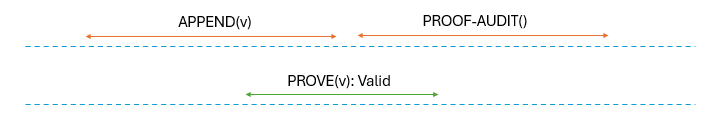
\includegraphics[width=1\linewidth]{ADLvsDL.png}
    \caption{
    \textit{DL} doesn't imply \textit{ADL}. In \textit{ADL} the PROOF-AUDIT must output the proof since the PROVE operation must be linearized before the APPEND which is linearized before the PROOF-AUDIT. However in \textit{DL}, the PROOF-AUDIT doesn't necessarily have to output the proof since the PROVE operation can be linearized after it (we simply set the "progress point" of the APPEND after the PROVE linearization).
    }
\end{figure}

The proof of Theorem~\ref{thm:ADLEquivelancy} is located at Appendix~\ref{prf:ADLEquivelancy}. The theorem implies that \textit{ADL} is no weaker than its original definition. Moreover, unlike last time we claim that it is \textbf{strictly stronger} in terms of its required synchronicity. The exact statement is given by Theorem~\ref{thm:ADLLowerBound}. Obviously, a lower bound of the consensus number of \textit{DL} implies a lower bound for the consensus number of \textit{ADL}. More specifically, \cite{AccessControl} provides a lower bound of $k$ for \textit{DL} in the case where $\vert\Pi_V\vert=\vert\Pi_M\vert=\vert\Pi_A\vert=k$. This lower bound directly applies to \text{ADL}. As we will see later in Theorem~\ref{thm:DLLowerBound}, we can strengthen this lower bound for \textit{DL} to hold even in the case where there is only a single manager. 

Figure~\ref{fig:ADLvsAL} displays an example where converse of Theorem~\ref{thm:ADLEquivelancy} doesn't hold. As we will prove later in Theorem~\ref{thm:ADLLowerBound}, this difference leads to a difference in the synchronization power of the objects.

We note here that \cite{AccessControl} provides an implementation of \textit{DL} using R/W objects and a $k$-consensus object where $k=\vert\Pi_V\vert$. However, by Theorem~\ref{thm:ADLLowerBound} it is impossible for this implementation to satisfy the properties of \textit{ADL}. An open question that remains is how large is the synchronization gap between \textit{DL} and \textit{ADL}?

To bridge the gap we suggest the definition of a \textit{Half-Atomic-DenyList} object (\textit{HADL} in short). 

\begin{definition}\label{def:ADL}[\textit{Half-Atomic-DenyList} definition, \textit{HADL} in short]
We alter the \textit{\mbox{PROVE} Validity} property as follows:
\begin{itemize}
   \item \textit{Weak-Completeness}. If there exists a valid \mbox{APPEND}(v) operation in $H'$ that completes before the invocation of a \mbox{PROVE}(v) operation in $H'$ by some $p\in \Pi_V$ then the prove operation must be invalid.
  \item \textit{Strong-Accuracy}. If the invocation of \mbox{PROVE}(v) by process $p$ is invalid then either $p\notin \Pi_V$ or there exists a preceding valid APPEND(v) operation in $\pi$.
\end{itemize}
\end{definition}

It is easy to see that \textit{ADL} is stronger than \textit{HADL} and that \textit{HADL} is stronger than \textit{DL}. We will later claim in Theorem~\ref{thm:HADLUpperBound} that the aforementioned upper bound on the consensus number of \textit{DL} can be applied directly on \textit{HADL}. This will imply that \textit{HADL} has a consensus number of $k$ where $k=\vert\Pi_V\vert$.

Lastly, our final result regards the \textit{Auditable Register} object. \cite{AuditableRegs} provides an implementation of \textit{AtomicAudit} using CAS and swap objects. It remains an open question whether there exists a better implementation that provides a tight upper bound to its consensus number.
To this end, in definition~\ref{def:HAA} we propose a slight relaxation of the \textit{AtomicAudit} object. This new definition gives way for an efficient implementation of the object, upper bounding its consensus number by the number of readers in the system.

\begin{definition}
    \label{def:HAA}
    The \textit{HalfAtomicAudit} object (\textit{HAA} in short) is defined like \textit{AtomicAudit} with the exception of the following \textit{READ Validity} relaxation:
    \begin{itemize}
        \item \textit{READ Validity}.
        \begin{itemize}
               \item \textit{Weak-Completeness}. If there exists a \mbox{WRITE}(v) operation in $H'$ (dentoed by $op_w$) that completes before the invocation of a \mbox{READ}() operation in $H'$ (denoted by $op_r$), then the $op_r$ operation must return a value written by some WRITE operation that coincides with or follows $op_w$ in $\pi$.
  \item \textit{Strong-Accuracy}. If the invocation of \mbox{READ}() returns value $v$ then there exists a preceding WRITE(v) operation in $\pi$.
        \end{itemize}
    \end{itemize}
\end{definition}


\section{Consensus Number Lower Bound of \textit{DL} and \textit{ADL}}
\subsection{Single-Auditor DL Lower bound}


\cite{AccessControl} showed that DenyList (and consequently \textit{ADL}) has a consensus number of at least $k$ where $\vert\Pi_V\vert=\vert\Pi_M\vert=\vert\Pi_A\vert=k$. The following theorem proves that DenyList (and consequently \textit{ADL}) has a consensus number of at least $k$ even when there is only a single manager.

The algorithm presented in the following theorem integrates the techniques presented in article \cite{AuditableRegs} for $k$-consensus using audible registers into the \textit{DL} model, demonstrating how these methods can effectively be applied. This result is quite surprising considering that DL registers differ from audible registers in the sense of atomicity. \textit{DL} registers do not promise the atomicity of a prove following an append operation, where audible registers do promise the atomicity of a read following a write operation. Nonetheless, by adjusting the mentioned algorithm for audible registers to the \textit{DL} model, we still manage to receive an algorithm with the same required properties.

\begin{theorem} \label{thm:DLLowerBound}
    Algorithm~\ref{alg:DLLowerBound} wait-free implements a k-consensus object using only R/W registers and DenyList objects with $\vert\Pi_M\vert=1, \vert\Pi_V\vert=\vert\Pi_A\vert=k$.
\end{theorem}

\begin{lemma}
  Algorithm~\ref{alg:DLLowerBound} satisfies Termination.
\end{lemma}
\begin{proof}
Let us fix some admissible execution of the algorithm. Consider some correct process $p_i$. Using the \textit{Termination} property of DenyList we know that all operations invoked by $p_i$ are followed by a response. Obviously, all loops in PROPOSE other than the \textit{loop 1} (lines 3-5) are iterated a finite amount of times. Additionally, the \textit{Progress} property of DenyList ensures that \textit{loop 1} consists of a finite amount of iterations since an APPEND(0) is invoked on $DenyLists[i]$ prior to the loop.
\end{proof}
\begin{lemma}
  Algorithm~\ref{alg:DLLowerBound} satisfies Validation.
\end{lemma}
\begin{proof}
We start by proving that if process $p_i$ reaches the return statement, then its value of \textit{safe\_values} is not empty. 

Let $p_k$ be the first process that exits \textit{loop 1}. Every process $p_i$ must complete \textit{loop 1} before proving on $DenyLists[j]$ for $j\neq i$. This implies that when $p_k$ exits \textit{loop 1}, $DenyLists[k]$ received proofs only from $p_k$. Additionally, when $p_k$ exits \textit{loop 1} this implies that it failed the PROVE(0) operation of line 4. From the \textit{No-Flickering} property we conclude that after that point, all other PROVE(0) operations are invalid. Therefore \textit{DenyLists[k].ProofAudit()} will contain only proofs of $p_k$. Therefore $p_i$ will add $Values[k]$ to its \textit{safe\_values} set at line 11.

We now move on to prove that \textit{safe\_values} contains only values proposed by some process. In other words, we must show that when $Values[j]$ is appended to \textit{safe\_values} at line 11 by some process $p_i$, then $Values[j] \neq \bot$.

If process $p_i$ appends $Values[j]$ to its \textit{safe\_values}, then we know that the \textit{DenyLists[j].ProofAudit()} operation (line 9) returned only $p_j$ proofs. More specifically, it contains no proofs of $p_i$. Using the \textit{PROOF-AUDIT Validity} property, we conclude that the \textit{DenyLists[j].Prove(0)} operation (line 7) performed by $p_i$ is invalid. By the \textit{Correctness} property, a \textit{DenyLists[j].Append(0)} operation must have occured prior. In other words, process $p_j$ must have executed line 2 beforehand. From here we conclude that $p_j$ executed $Values[i] \leftarrow v$ (line 1) beforehand.
    
\end{proof}


\begin{algorithm}
    \caption{A $k$-consensus implementation using DenyList objects with $\vert\Pi_M\vert=1$ and $\vert\Pi_V\vert=\vert\Pi_A\vert=k$.}
    \label{alg:DLLowerBound}
    \begin{algorithmic}[1]
    \Statex \textbf{Shared Variables:}
    \Statex \hspace{1em} \textit{DenyLists}: A $k$-Dimensional array of $k$-DenyList objects. Each object has a different writer.
    \Statex \hspace{1em} \textit{Values}: A $k$-Dimensional array of R/W registers, initially $\{\bot\}^k$.

    \Statex
    \Statex \textbf{Local Variables:} \hfill \text{ \textbf{Pseudo code for $p_i,i\in [0,k-1]$}}
    \Statex \hspace{1em}\textit{safe\_values}: A set. Initially $\emptyset$
    \Statex \hspace{1em}\textit{proofs}: A set. Initially $\emptyset$

    \Statex
    \Statex \textbf{Operation} PROPOSE(v) \textbf{is}
    \State $Values[i] \leftarrow v$;
    \State $DenyLists[i].Append(0)$;
    \Repeat
    \State $ret \leftarrow DenyLists[i].Prove(0)$;
    \Until $ret \neq false$;
    \For{$j = 0$ \textbf{to} $k - 1$}
        \State $DenyLists[j].Prove(0)$;
    \EndFor
    \For{$j = 0$ \textbf{to} $k-1$}
        \State $proofs\leftarrow DenyLists[j].ProofAudit()$;
        \If{$proofs$ contains only proofs from $p_j$}
            \State ${safe\_values}.add(Values[j])$
        \EndIf
    \EndFor

    \State \textbf{return} min\{\mbox{safe\_values}\}
    \end{algorithmic}
\end{algorithm}
\begin{lemma}
  Algorithm~\ref{alg:DLLowerBound} satisfies Agreement.
\end{lemma}



\begin{proof}
We prove that all process that reach the return statement have the same set \textit{safe\_values}. To do so we prove the following claim: For any two process $p_i,p_j$, $p_j$'s \textit{safe\_values} contains $p_i$'s \textit{safe\_values}.

Let $v$ be a value in $p_i$'s \textit{safe\_values}. This value equals to some $Values[k]$ value which corresponds to some PROOF-AUDIT operation by $p_i$ on $DenyLists[k]$ that returns only proofs of $p_k$. We separate by cases: 

\begin{itemize}
    \item If $p_i$ invokes PROOF-AUDIT on $DenyLists[k]$ after $p_j$ invokes PROOF-AUDIT on $DenyLists[k]$ then this trivially implies that $p_j$'s invocation also returns only $p_k$ proofs, and thus $p_j$ adds $v$ to its  \textit{safe\_values}. 
    \item If $p_i$ invokes PROOF-AUDIT on $DenyLists[k]$ before $p_j$ invokes PROOF-AUDIT on $DenyLists[k]$ then we need to prove that all PROVE(0) operations on $DenyLists[k]$ are invalid between the two PROOF-AUDIT operations. This will conclude the case, since  $p_j$'s and $p_i$'s PROOF-AUDIT operations on $DenyLists[k]$ will return the same. Consider the point in time where $p_i$ invokes PROOF-AUDIT on $DenyLists[k]$. Prior to that $p_i$ failed a PROVE(0) operation on  $DenyLists[k]$ and using the \textit{No-Flickering} property we infer that from that point in time all PROVE(0) operations on $DenyLists[k]$ are invalid.

\end{itemize}
. 
\end{proof}


\subsection{Single-Manager Single-Prover Single-Auditor ADL Lower bound}

In this section we prove that \textit{ADL} is \textbf{strictly} stronger than DenyList in terms of required-synchronicity. The following theorem states that a single-manager single-prover single-auditor ADL register has a consensus number of at least 2. This is in contrast with \cite{AccessControl} that upper bounded DenyList's consensus number by the number of its provers. 

Similarly to \textit{Algorithm~\ref{alg:DLLowerBound}}, the following algorithm utilizes the techniques presented in \cite{AuditableRegs} for 2-consensus using 2 audible registers. Each register is configured to be a single-writer single-reader single-auditor, corresponding respectively to a single-manager single-prover single-auditor ADL register.

\begin{theorem}\label{thm:ADLLowerBound}
        Algorithm~\ref{alg:ADLLowerBound} wait-free implements a 2-consensus object using only R/W registers and DenyList objects with $\vert\Pi_M\vert=\vert\Pi_V\vert=\vert\Pi_A\vert=1$.
\end{theorem}

\noindent The following algorithm could not be generalized to \textit{DL} registers, since it relies on the atomicity of the \textit{ADL} register, which mandates that a proof is immediately invalidated after being appended to the \textit{ADL}. The \textit{ADL} model is inspired by the audible registers model, which guarantees the atomicity of reads immediately following writes.

\begin{lemma}
  Algorithm~\ref{alg:ADLLowerBound} satisfies Termination.
\end{lemma}

\begin{proof}
Using the \textit{Termination} property of \textit{ADL} we know that all invocations of \textit{ADL} methods eventually return. Besides those methods invocations, all other operations are finite, therefore the whole algorithm is promised to terminate.
\end{proof}
\begin{lemma}
  Algorithm~\ref{alg:ADLLowerBound} satisfies Validity.
\end{lemma}
\begin{algorithm}
    \caption{A $2$-consensus implementation using DenyList objects with $\vert\Pi_M\vert=\vert\Pi_V\vert=\vert\Pi_A\vert=1$.}.
    \label{alg:ADLLowerBound}
    \begin{algorithmic}[1]
    \Statex \textbf{Shared Variables:}
    \Statex \hspace{1em} \textit{DenyLists}: A $2$-Dimensional array of DenyList objects. The i'th object has auditor/manger $p_i$ and has prover $p_{1-i}$.
    \Statex \hspace{1em} \textit{Values}: A $2$-Dimensional array of R/W registers, initially $\{\bot\}^k$.

    \Statex
    \Statex \textbf{Local Variables:} \hfill \text{ \textbf{Pseudo code for $p_i,i\in [0,1]$}}
    \Statex \hspace{1em}\textit{proofs}: A set. Initially $\emptyset$

    \Statex
    \Statex \textbf{Operation} PROPOSE(v) \textbf{is}
    \State $Values[i] \leftarrow v$;
    \State $DenyLists[i].Append(0)$;
    \State $res\leftarrow DenyLists[1-i].Prove(0)$;
    \State $proofs\leftarrow DenyLists[i].ProofAudit()$;
    \If{$proofs = \emptyset$ and $res\neq false$}
        \State\textbf{return} $Values[i]$
    \EndIf
    \If{$proofs \neq \emptyset$}
        \State\textbf{return} $Values[1-i]$
    \EndIf
    \State \textbf{return} min\{$Values[i],Values[1-i]$\}
    \end{algorithmic}
\end{algorithm}

\begin{proof}
If $p_i$ returns $Values[i]$ (lines 6, 9), then validity holds since $p_i$ previously wrote its proposed value $v$ to $Values[i]$. Otherwise, if $p_i$ returns $Values[1-i]$ (lines 8, 9) then it didn't fulfill the constraints of line 5. Therefore, $res=false$ and his prove in line 3 failed, meaning that $p_{(1-i)}$ have appended in line 2 beforehand due to the \textit{Correctness} of \textit{ADL}. Finally, by the order of execution, $p_{(1-i)}$ writes its proposed value $v_{(1-i)}$ to $Values[1-i]$ in line 1 before $p_i$ executes line 3, and as a result $p_i$ will return $v_{(1-i)}$. Thus, the algorithm satisfies \textit{Validity}.
\end{proof}

\begin{lemma}
  Algorithm~\ref{alg:ADLLowerBound} satisfies Agreement.
\end{lemma}

\begin{proof}
We cover all cases for process $p_i$ to return a value:

\begin{itemize}
    \item \textbf{Case 1.} If $p_i$ returns in line 6, it returns its own proposed value $v_i$ (by validity). Moreover, the statement in line 5 is true, meaning $p_i$ made a valid proof in line 3. Due to the \textit{Strong-Accuracy} and \textit{Strong-Completeness} of \textit{ADL}, then $p_{(1-i)}$ appends in line 2 after $p_i$ proves in line 3. Consequently, $p_{(1-i)}$ has $p_i$'s valid proof in the $proofs$ set when executing line 4 (thanks to the \textit{PROOF\_AUDIT Validity}). Finally, $p_{(1-i)}$ will return in line 7, which contains $v_i$ as well by validity.
    
    \item \textbf{Case 2.} If $p_i$ returns in line 8, it returns $v_{(1-i)}$ (by validity). Moreover, the statement in line 5 is true, meaning $p_{(1-i)}$ made a valid proof in line 3, so $p_{(1-i)}$ proved in line 3 before $p_i$ appended in line 2 (by \textit{Strong-Accuracy} and \textit{Strong-Completeness}). Therefore, $p_i$'s proof in line 3 will be invalid since $p_{(1-i)}$ already appended in line 2 by then. Consequently, when $p_{(1-i)}$ executes line 5, his ${proofs}$ set is empty (by \textit{PROOF\_AUDIT Validity}), and {res=true}, meaning it also returns $v_{(1-i)}$ by validity.

    \item \textbf{Case 3.} If $p_i$ returns in line 9, it returns \textit{min\{$Values[i],Values[1-i]$\}}. Moreover, both statements in lines 5,7 are incorrect, meaning $proofs=\emptyset$ and $res=false$. Therefore, $p_{(1-i)}$ receives an empty $proofs$ set in line 4 (by \textit{PROOF\_AUDIT Validity}). Also, $p_{(1-i)}$ fails in proving in line 3 - assume in contradiction that it made a valid proof, then $p_i$ executed line 2 after $p_{(1-i)}$ executed line 3 (by \textit{Strong-Accuracy} and \textit{Strong-Completeness}). This implies that $p_i$ would have gotten $p_{(1-i)}$'s proof in line 4 (by \textit{PROOF\_AUDIT Validity}), in contradiction to it being empty. Finally, since  $p_{(1-i)}$ $proofs$ set is empty and $res=false$, it returns \textit{min\{$Values[i],Values[1-i]$\}} as well.

\end{itemize}

\end{proof}

\section{Consensus Number Upper Bounds of \textit{DL}, \textit{ADL} and \textit{HADL}}
\subsection{\textit{HADL} Upper Bound}
In the following section we prove that the consensus upper bound provided in \cite{AccessControl} for \textit{DenyList} also applies for the stronger definition of \textit{HADL}. This result provides further justification for the definition of \textit{HADL}.

\begin{theorem}
\label{thm:HADLUpperBound}
    Algorithm 3 from \cite{AccessControl} wait-free implements a \textit{HADL} object with $\vert\Pi_V\vert=k$ using only $k$-consensus objects and R/W registers.
\end{theorem}

\begin{proof}
    Since we know that Algorithm 3 from \cite{AccessControl} implements \textit{DL}, in order to prove that it implements \textit{HADL} we only need to prove that it satisfies the \textit{Weak-Completeness} property, since all other properties are syntactically equivalent. 
    
    Suppose a valid \mbox{APPEND}(v) operation invoked by $p'\in\Pi_M$ completes in $H'$ before the invocation of some  \mbox{PROVE}(v) operation by some $p\in \Pi_V$. In this scenario, the \textit{AS-LV} object contains the value $v$ prior to the invocation of PROVE(v). Let $((cnt,p),C_v)$ represent the value appended to \textit{AS-Queue} at line 10 of the PROVE(v) operation.
    Now consider the tuple $(winner,val)$ of line 15 in the case where $winner=((cnt,p),C_v)$. We claim the $val$ must contain $v$. This is because the tuple $(winner,val)$ is proposed by some process $p^*\in\Pi_M$. When $p^*$ sets the value of $val$ at line 14, we know that the \textit{AS-LV} object contains the value $v$, since this moment occurs after the invocation of \mbox{PROVE}(v) (otherwise $((cnt,p),C_v)$ isn't in the queue at that time, and $p^*$ cannot suggest it a $winner$). thus $val$ must contain $v$, rendering the PROVE(v) operation invoked by p invalid. This ensures that the \textit{Weak-Completeness} property is maintained.
\end{proof}

\begin{corollary}
\textit{HADL} has a consensus number of k where $\vert\Pi_V\vert = k$.
\end{corollary}

\subsection{Single-Auditor Single-Manager \textit{ADL} Upper Bound}

Before presenting the upper bound, we must define the following utility register \textit{snapshot\&modify}. This register holds an array of $n$ values, where each of the values $i\in [n]$ has a unique writer $p_i$. Any \textit{snapshot\&modify} register $R$ must support the two following atomic operations:
\begin{itemize}
    \item \textit{R.Fetch\&localModify}(v): When invoked by process $p_i$ this operation returns a snapshot of all values and sets the $i$'th value to $v$. 
    \item \textit{R.Snapshot}($v_1,\ldots,v_n$): This operation returns a snapshot of all values.
\end{itemize}

Later on we will see how this object is useful for implementing single-auditor single-manager \textit{ADL}. Before that we claim that the consensus number of \textit{snapshot\&modify} is 2. To do so, we will implement \textit{snapshot\&modify} using a register that supports operations $read$ and $fetch\&add$. As claimed in \cite{herlihy1991wait}, a register that supports operations $read$ and $fetch\&add$ has a consensus number of 2. Thus theorem~\ref{thm:sm} will imply our claim.

We can encoded $n$ unbounded values $v_1,\ldots,v_n$ in a single value $v$ as follows: Value $i$ is composed from bits $i,i+n,i+2n,\ldots$ of $v$. We can define \textit{GetValues}(v) to return the array of $v_1,\ldots,v_n$ encoded in $v$. Additionally, we can define \textit{EncodeValue($v_1,\ldots,v_n$)} to return the encoded value $v$.

\begin{theorem}
    \label{thm:sm} Algorithm~\ref{alg:sm} implements \textit{snapshot\&modify} using only a register that supports operations $read$ and $fetch\&add$.
\end{theorem}


\begin{proof}
    Let us fix an execution of the algorithm and let $H$ be its history. Let $H'$ be the completed version of $H$ that is obtained by the completing all pending operation that have passed their linearization point (to be defined) and discarding the rest. 
    
    We set the $fetch\&add$ operation of line 6 to be the linearization point of \textit{Fetch\&LocalModify}. We set the $Read$ operation of line 8 to be the linearization point of \textit{Snapshot}. In the implementation, $R$ contains the encoded value of $v_1,\ldots,v_n$. Hence, line 8 returns the values of $v_1,\ldots,v_n$ at the point of \textit{Snapshot}'s linearization. For the same reason, line 6 returns the values of $v_1,\ldots,v_n$ at the point of \textit{Fetch\&LocalModify}'s linearization. Finally, we claim that $v_i$ changes its value atomically to $x$ at \textit{Fetch\&LocalModify}'s linearization point (the $fetch\&add$ operation) and all other values remain the same. This is since by definition $GetValues(add\_val + a)[j]$ equals $GetValues(a)[j]$ for all $a$ and $j\neq i$ (and thus only $v_i$ changes). Additionally, since by definition $GetValues(add\_val + curr\_encoded\_val)[i]=x$ and since the bits of $R$ regarding $v_i$ don't change between $curr\_encoded\_value$ and the \textit{fetch\&add} operation, we conclude that the resulted encoded value of the \textit{fetch\&add} operation encodes $v_i$ as $x$. 
\end{proof}

\begin{algorithm}
    \caption{A wait-free implementation of \textit{snapshot\&modify} only a register that supports operations $swap$ and $fetch\&add$.}
    \label{alg:sm}
    \begin{algorithmic}[1]
          
    \Statex \textbf{Shared Variables:}
    \Statex \hspace{1em} \textit{R}: A register accessed with \textit{read} and \textit{fetch\&add} primitives. Initially equals \mbox{\textit{EncodeValue}(${v_i}_1,\ldots,{v_i}_n$)}.
    
    \Statex
     \State \textbf{Operation} FETCH\&LOCAL\_MODIFY(x) \textbf{is}  \hfill \text{ \textbf{Pseudo code for $p_i,i\in [0,n-1]$}}
     \State $curr\_encoded\_val = R.Read()$;
     \State $v_1,\ldots,v_n \leftarrow GetValues(curr\_encoded\_val)$;
     \State $v_i \leftarrow x$;
     \State $add\_val \leftarrow EncodeValue(v_1,\ldots,v_n) - curr\_encoded\_val$;
     \State \textbf{return} $R.fetch\&add(add\_val)$;

     \Statex
     \State \textbf{Operation} SNAPSHOT() \textbf{is}
     \State \textbf{return} $GetValues(R.Read())$;
    \end{algorithmic}
\end{algorithm}

We now move on to implement single-auditor single-manager \textit{ADL} using only R/W and \textit{snapshot\&modify} registers (Theorem~\ref{thm:ADLUpperBound}). This will imply a consensus number upper bound of 2, matching the lower bound proven in the previous section.

\begin{corollary}[of Theorem~\ref{thm:ADLUpperBound}]
    The single-auditor single-manager \textit{ADL} object has a consensus number of 2.
\end{corollary}

Interestingly enough, this result also implies an upper bound of single-auditor single-manager \textit{DenyList}. This expands our understanding of the synchronicity requirements of \textit{DenyList}, which until now only a consensus number upper bound of $\vert\Pi_V\vert$  was known.

\begin{corollary}[of Theorem~\ref{thm:ADLUpperBound}]
    The single-auditor single-manager \textit{DL} object has a consensus number of at most 2.
\end{corollary}

The following algorithm (Algorithm~\ref{alg:ADLUpperBound}) lightly resembles that of the single-auditor \textit{AtomicAudit} implementation of \cite{AuditableRegs}. However algorithm~\ref{alg:ADLUpperBound} exhibits some crucial differences that are necessary adjustments of the implementation to meet the requirements of \textit{ADL}.
\begin{theorem}
    \label{thm:ADLUpperBound}  
    Algorithm~\ref{alg:ADLUpperBound} wait-free implements an \textit{ADL} object with a single manager and single auditor and a general amount of provers using only \textit{snapshot\&modify} and R/W registers.
\end{theorem}

\begin{algorithm}
\footnotesize % or \scriptsize, \tiny

    \caption{A wait-free implementation of \textit{ADL} with a single manager, a single auditor and $k$ provers using \textit{Snapshot\&modify}.}
    \label{alg:ADLUpperBound}
    \begin{algorithmic}[1]
    
    \Statex \textbf{Shared Variables:}
    \Statex \hspace{1em} \textit{R}: A \textit{Snapshot\&modify} object of $k+1$ values $v_0,\ldots,v_{k-1},\mathcal{A}$. Process $p_i$ is the writer of value $v_i$. Process $p_m$ is the writer of $\mathcal{A}$. Initially $\{(0, \bot)\}^{k}\circ\{\emptyset\}$.
    \Statex \hspace{1em} \textit{Proofs}:  A $k$-Dimensional array of R/W registers, initially $\{\emptyset\}^k$.

    
    \Statex
    \Statex \textbf{Local Variables:} \hfill \text{ \textbf{Pseudo code for prover $p_i,i\in [0,k-1]$}}
    \Statex \hspace{1em} \textit{counter}: A positive integer, initially $1$.
    
    \Statex
    \Statex \textbf{Operation} PROVE(v) \textbf{is}
    \If{$p_i \notin \Pi_V$}
    \State \textbf{return} false;
    \EndIf
    \State $\mathcal{A} \leftarrow \textit{R.Fetch\&LocalModify}((counter,v))[m]$;
    \If{$v \notin \mathcal{A}$}
    \State $\pi_{SNM} \leftarrow Proof(v,\mathcal{A}$);
    \State $Proofs[i].add((\pi_{SNM},p_i,counter))$;
    \State $counter\leftarrow counter+1$;
    \State \textbf{return} $\pi_{SNM}$;
    \Else
        \State \textbf{return} false;
    \EndIf

    \Statex
        \Statex \textbf{Local Variables:} \hfill \text{ \textbf{Pseudo code for manager/auditor $p_m$}}
    \Statex \hspace{1em} \textit{audit\_result}: Initially  $\emptyset$.
    \Statex
    \Statex \textbf{Operation} APPEND($v$) \textbf{is} 
    \If{$p_m \notin \Pi_M$ \textbf{or} v$\notin \mathcal{S}$}
    \State \textbf{return} false;
    \EndIf
    \State $\mathcal{A}$$\leftarrow R.Snapshot()[m]\cup\{v\}$;
    \State $v_0,\ldots,v_{k-1},\mathcal{A}\leftarrow$\textit{R.Fetch\&LocalModify}($\mathcal{A}$);
        \For{$i=0$ \textbf{to} $k-1$}
    \State $value, counter\leftarrow v_i$;
    \If{counter=0}
    \State \textbf{continue};
    \EndIf
    \State $proofs\leftarrow$first $(counter-1)$ proofs of $Proofs[i]$;
    \If{$value \notin \mathcal{A}$}
    \State $\pi_{SNM} \leftarrow Proof(value,\mathcal{A}$);
    \State $proofs.add((\pi_{SNM},p_j,counter))$;
    \EndIf
    \State \textit{audit\_result}$.add(proofs)$;\hfill \text{ \textit{//don't add duplicates, i.e. don't add if $(p_j,counter)$ proof already exists.}}
    \EndFor 
    \State \textbf{return} v;

    \Statex

    \Statex \textbf{Operation} PROOF\_AUDIT() \textbf{is} 
        \If{$p_a \notin \Pi_A$}
    \State \textbf{return} false;
    \EndIf
    \State $v_0,\ldots,v_{k-1},\mathcal{A}\leftarrow R.Snapshot()$;
    \For{$i=0$ \textbf{to} $k-1$}
    \State $value, counter\leftarrow v_i$;
    \If{counter=0}
    \State \textbf{continue};
    \EndIf
    \State $proofs\leftarrow$first $(counter-1)$ proofs of $Proofs[i]$;
    \If{$value \notin \mathcal{A}$}
    \State $\pi_{SNM} \leftarrow Proof(value,\mathcal{A}$);
    \State $proofs.add((\pi_{SNM},p_j,counter))$;
    \EndIf
    \State \textit{audit\_result}$.add(proofs)$;\hfill \text{ \textit{//don't add duplicates, i.e. don't add if $(p_j,counter)$ proof already exists.}}
    \EndFor 
    \State \textbf{return} \textit{audit\_result};
    \end{algorithmic}
\end{algorithm}

\begin{proof}
    Let us fix an execution of the algorithm and let $H$ be its history. Let $H'$ be the completed version of $H$ that is obtained by the completing all pending operation that have passed their linearization point (to be defined) and discarding the rest. 

    For all operations PROVE, APPEND, PROOF\_AUDIT, if they are invalid in terms of their sanity checks (AKA the conditional of lines 1,11,25 respectively) we set their linearization point to be their point of return. Otherwise, We set the \textit{Fetch\&LocalModify} operator of line 3 to be the linearization point of PROVE, the \textit{Fetch\&LocalModify} operator of line 14 be the linearization point of APPEND and finally the \textit{Snapshot} operation of line 27 be the linearization point of PROOF\_AUDIT. We totally order all completed operations by the order of their linearization point executions and construct sequential history $\pi$ accordingly.

    Trivially, the \textit{Termination} property is satisfied since all loops are finite. Secondly, the \textit{APPEND Validity} property is implied from the condition of line 11. The optional \textit{Anonymity} property is also satisfied if the generated proofs are zero-knowledge, and therefore no additional information can be gleaned from a READ() operation. 
    We move on to prove the \textit{PROVE validity} property.

    \begin{lemma}
        Algorithm~\ref{alg:ADLUpperBound} satisfies \textit{PROVE validity}.
    \end{lemma}
    \begin{proof}
        Suppose there exists a valid APPEND(v) operation $op_a$ that precedes a PROVE(v) operation $op_v$ in $\pi$. We claim that $op_v$ is invalid. If $op_v$ is invalid in terms of its sanity check, then we are done. Otherwise, we know that the \textit{Fetch\&LocalModify} operation of line 14 of $op_a$ occurs before the  \textit{Fetch\&LocalModify} operation of line 3 of $op_v$. Thus, we know that when we reach the \textit{Fetch\&LocalModify} operation of line 3 of $op_v$, the $m$'th value of $R$ (denoted by $\mathcal{A})$ must contain $v$. This causes the conditional of line 4 to fail, causing $op_v$ to return false, rendering $op_v$ invalid. Thus the algorithm satisfies \textit{Strong-Completeness}.

        Next consider some invalid PROVE(v) operation $op_v$. Then, either $p\in\Pi_v$ or it returns false on line 10. We claim that in the second case, there must exist a preceding valid APPEND(v) operation in $\pi$, proving the \textit{Strong-Accuracy} property. Since $op_v$ returns false, we know that when it invoked the \textit{Fetch\&LocalModify} operation of line 3,  the $m$'th value of $R$ (denoted by $\mathcal{A})$ must have contained $v$. This means that beforehand some valid APPEND(v) operation $op_a$ must have executed its \textit{Fetch\&LocalModify} operation of line 14. Therefore $op_a$ precedes $op_v$ in $\pi$, proving \textit{Strong-Accuracy}.
    \end{proof}
    
    We move on to prove the \textit{PROOF\_AUDIT validity} property.

    \begin{lemma}
        Algorithm~\ref{alg:ADLUpperBound} satisfies \textit{PROOF\_AUDIT validity}. 
    \end{lemma}

    \begin{proof}
        Note that every proof of $audit\_result$ is either taken from some $Proofs[i]$, generated by prover $p_i$ at line 6, or generated by $p_m$ in operation APPEND/PROOF\_AUDIT at lines 22, 35 respectively. We first claim that the proofs generated by $p_m$ "fast-forward" some proof of prover $p_i$. Formally, if $p_m$ adds entry $(\pi_{SNM},p_i,counter)$ to $audit\_result$ then at its linearization point there must be a concurrent in-progress valid  PROVE(v) operation $op_v$ that is supposed to add that exact entry to $Proofs[i]$ (and additionally $op_v$ has already executed its linearization point). First notice that when $p_m$ executes its linearization point, some valid PROVE operation of $p_i$ must have executed \textit{R.Fetch\&LocalModify((counter,v))} of line 3, (since the value $value$ is valid, and must have been written by some valid PROVE operation to $R$), but no PROVE operation of $p_i$ has yet to add a proof with count $counter$ on line 6 (since $p_m$ doesn't add duplicates). This means that there must exist some valid $op_v$ operation that executed line 3 but not line 6 at the point of $p_m$'s linearization. Moreover, the value of $\mathcal{A}$ at $op_v$ (line 3) must be the same as that of $p_m$'s operation (line 14,27 respectively), since the value of $p_m$ in $R$ cannot change between the two points in time - if it did change, then this implies that a different APPEND operation occured between the two points in time, and if that was the case then it would have "fast-fowarded" the proof of $op_v$ instead. This implies that $p_m$ generates the exact same proof as prover $p_i$ intends to.

        Now using this claim, it is easy to see why  \textit{PROOF\_AUDIT validity} holds.
        
        Let $op_v$ be a valid PROVE(v) operation of process $p_i$ that precedes some valid PROOF\_AUDIT() operation $op_a$. This means that the \textit{Fetch\&LocalModify} operation of line 3 of $op_v$ occurs before the \textit{Snapshot} operation of line 27 of $op_a$. 
        Let $counter_v$ be the value of $counter$ at line 3 of $op_v$ and let $counter_a$ be the value of counter fetched from $v_i$ at line 29 of $op_a$. Then since $counter$ only increases per prover we know that $counter_a\geq counter_v$. If $counter_a > counter_v$ then this means that when we reach the \textit{Fetch\&LocalModify} operation of line 14 of $op_a$, operation $op_v$ must have completed since a new PROVE operation of $p_i$ has started after it. More specifically, $op_v$ must have executed line 6 and thus $op_a$ adds the associated proof of $op_v$ to $audit\_result$ (if it wasn't added already by some previous operation). Otherwise, $counter_a = counter_v$. This implies that the $value$ variable of line 29 of $op_a$ equals $v$ since $op_v$ is valid. Moreover, since $op_v$ is valid then using our claim $op_a$ adds the associated proof of $op_v$ to $audit\_result$ (if it wasn't fast-forwarded already by some previous APPEND operation). In total we get that $op_a$ returns the associated proof of $op_v$.

        Finally, using our claim, it is easy to see that every proof outputted by some PROOF\_AUDIT operation $op_a$ corresponds with some PROVE operation that precedes $op_a$ in $\pi$. This is because every entry in $audit\_result$ is either generated by some PROVE operation $op_v$ at line 6, and thus $op_v$ is clearly linearized before $op_a$, or is generated by some $p_m$ operation $op'$ via fast forwarding, which by our claim, there is a concurrent PROVE operation $op_v$ that precedes $op'$ in $\pi$.

    \end{proof}

    By that we conclude our proof of Theorem~\ref{thm:ADLUpperBound}, Algorithm~\ref{alg:ADLUpperBound} upholds all properties of \textit{ADL}.
\end{proof}


\section{Consensus Number Upper-Bound of \textit{HAA}}

Up to this point, we've showed results regarding the DenyList and its derivatives, while utilizing techniques shown in audible registers context. In this section we'll shift our focus to the audible registers. Similary, we'll show how techniques that were presented in the DenyList context can be applied to audible registers, while strengthening the connection between those two models.


More specifically, in following theorem we prove that \textit{HalfAtomicAudit} with $k$-readers and a general amount of writers/readers has consensus number $k$. The algorithm by which we achieve this result is a modified version of the $k$ consensus algorithm for DenyList presented in \cite{AccessControl}.

\begin{theorem}
    Algorithm~\ref{alg:auditableRegs} wait-free implements an \textit{HalfAtomicAudit} register with $k$-readers and a general amount of writers/auditors.
\end{theorem}

\begin{proof}


First, we prove that Algorithm~\ref{alg:auditableRegs} satisfies \textit{Termination}. Both WRITE and READ operations obviously terminate as a result of the atomicity of \textit{R/W} registers and \textit{Atomic-Snapshot} objects. The crucial step in showing the termination of the READ operation is to show that the while loop has a finite amount of iterations. The relation $\mathcal{R}$ creates a strict order between accesses to the \textit{ASQueue}, where in each iteration the winner is being added to the \textit{evaluated} array, and gets removed from the snapshot of \textit{ASQueue}. Assume in contradiction there exists a process $p_i$ which has a value $v$ in its $queue$ that never gets chosen as a winner in the consensus, where $v$ is the oldest one in the execution to be so. This implies that $v$ is in $ASQueue$, and that it wasn't chosen yet, so no process holds it in its $evaluated$ collection. At some point, $v$ is the oldest value in all processes local $queue$ snapshot (since all previous values were evaluated), meaning that the consensus will eventually return $v$, due to the validity property, and it'll evaluated, in contradiction.

Let $H$ be the history of some execution $E$, and denote $H'$ as the completed history of $H$. In order to complete the unfinished operations, we present the linearization points: the linearization points of WRITE and AUDIT occur in lines 14, 15 respectively. The linearization point of the READ operation invocation is defined as the point where some process adds it to the \textit{ReadLogs} structure in line 9, meaning it was chosen as the winner of that round (happens eventually due to termination). Every operation that did not reach its linearization point yet can be ignored (not appear in H'). Otherwise, complete the READ invocation by returning the current $val$ it holds, and the AUDIT operation by returning the snapshot received. We build $\pi$ as the order between the execution of the linearization points.

The linearization property fulfills since: the WRITE and AUDIT operations obviously arrive their linearization points before returning, meaning every operation invoked after the WRITE and AUDIT operations finish, arrives its linearization points after them. Regarding the READ operation, it also arrives its linearization point before returning - since it writes itself to the $ReadLogs$ before returning (when chosen in consensus), therefore it has to be written before returning as well.\\

Finally, we prove the validity of the READ and AUDIT implementations. 

\begin{itemize}
\item READ \textit{Validity} - Initially we'll prove the \textit{Strong-Accuracy} property.  The value returned from a READ invocation must be a value chosen in line 7 using the consensus. All proposed values are read from \textit{CurrVal}, which is modified only by WRITEs invocations, therefore it is indeed a value that was written before. We move on to the \textit{Weak-Completeness} property. Assume there exists a WRITE(v) operation that completes before the invocation of a READ in $H'$. First, in each iteration of the while loop, the chosen value in the consensus is "getting newer", meaning there can't be some consensus iteration of index $i$, that yields an older version of $CurrVal$ of some following iteration of index $j>i$ (by means of WRITE invocations). This claim is correct since the consensus in every iteration is sampled before all processes sample $CurrVal$ again for the next round, so the next round consensus has to yield a newer version of the variable. Secondly, as we showed, there exists some iteration where the READ invocation in discussion is chosen as the winner in the consensus. At this point, we can be sure that the chosen $val$ was sampled from $CurrVal$ after that READ invocation have occurred. This value is assured to be updated by all WRITE invocations that finished before that READ has started, and could be even more updated by WRITE operations that started afterwards.

\item AUDIT \textit{Validity} - we start by showing \textit{Completeness}. Since the linearization point occurs on line 9, each READ operation that preceeds an AUDIT in $\pi$ will be written to $ReadLogs$ before the snapshot is taken. Because the snapshot object is promised to be atomic, the AUDIT will contain the mentioned read operation $(p,v)$. We now prove \textit{Strong Accuracy} - if the audit contains a pair $(p,v)$ then it was written by some process $p_2$, which corresponds to a READ invocation of process $p$. Since the linearization point occurs exactly when $p_2$ writes that pair into the $ReadLogs$, which occurred before the AUDIT snapshot was taken, then the READ invocation truly did come before the AUDIT in $\pi$.

\end{itemize}


\end{proof}

\begin{algorithm}
    \caption{A wait-free implementation of an auditable register with $k$-readers and a general amount of writers/auditors}
    \label{alg:auditableRegs}
    \begin{algorithmic}[1]
    
    \Statex \textbf{Shared Variables:}
    \Statex \hspace{1em} \textit{CurrVal}: A shared R/W register. Initially $\emptyset$.
    \Statex \hspace{1em} \textit{ASQueue}: An $k$-dimensions Atomic-Snapshot object, Initially $\{\emptyset\}^N$
    \Statex \hspace{1em} \textit{ConsArr}: An array of $k$-consensus objects of size $l>0$.
    \Statex \hspace{1em} \textit{ReadLogs}:  An $l$-dimensions Atomic-Snapshot object, Initially $\{\emptyset\}^l$
    
    \Statex
    \Statex \textbf{Local Variables:} \hfill \text{ \textbf{Pseudo code for reader $p_i$}}
    \Statex \hspace{1em} \textit{evaluated}: An array of size $l>0$, initially  $\{\emptyset\}^l$
    \Statex \hspace{1em} \textit{counter}: A positive integer, initially $0$.
    
    \Statex
    \Statex \textbf{Operation} READ() \textbf{is}
    \State $cnt \leftarrow counter$;
    \State $ASQueue.Update((cnt, p_i), p_i)$;
    \State $queue\leftarrow ASQueue.Snapshot() \setminus evaluated$;
    \While{$(cnt,p_i)\in Q$} 
        \State $oldest\leftarrow$ the smallest value in $queue$ under relation $\mathcal{R}$;
        \State $prop \leftarrow (oldest, CurrVal)$;
        \State $(winner, val) \leftarrow ConsArr[counter].Propose(prop)$;
        \State $(cnt_{p_w},p_w) \leftarrow winner$;
        \State $ReadLogs.Update((p_w, val), cnt_{p_w})$;
        \State $evaluated\leftarrow evaluated \cup \{winner\}$;
        \State $queue\leftarrow queue \setminus \{winner\}$;
        \State $counter \leftarrow counter + 1$
        % \If{$v == \bot$} 
        %     \State success = \textbf{true} \hfill \textit{// Success if CAS operation is successful}
        % \Else 
        %     \State $x = \textbf{GenerateNewValue}()$ \hfill \textit{// Generate a new value and retry}
        % \EndIf
    \EndWhile
    \State \textbf{return} val

    \Statex
    \Statex \textbf{Operation} WRITE($v$) \textbf{is} \hfill \text{ \textbf{Pseudo code for writer $p_i$}}
    \State $CurrVal \leftarrow v$


    \Statex
    \Statex \textbf{Operation} AUDIT() \textbf{is} \hfill \text{ \textbf{Pseudo code for auditor $p_i$}}
    \State \textbf{return} $ReadLogs.Snapshot()$

    \end{algorithmic}
\end{algorithm}


\section{Summary and Discussion}

In this article, we explored synchronization and auditability within distributed systems by examining two recently introduced but seemingly unrelated objects: the auditable register and Access-Control objects. We developed and presented new definitions, revealing the equivalences and distinctions between these models. Additionally, we established consensus number lower and upper bounds for the objects defined in our study and proved stronger bounds for previously established models in specific systems. However, several questions remain open:
\begin{itemize}
    \item Is there an efficient implementation of general \textit{AtomicAudit}? How large is the synchronization gap between \textit{AtomicAudit} and \textit{HAA}?

\item Is there an efficient implementation of general \textit{ADL}? How large is the synchronization gap between \textit{DL} and \textit{ADL}?
\end{itemize}

\bibliographystyle{plainurl}
\bibliography{citations}

\appendix
\section{Appendix}
\subsection{Proof of Theorem~\ref{thm:AALEquivelancy}}

\begin{proof}\label{prf:AALEquivelancy}
Let $H$ be the history of some execution of \textit{AAL}. Let $H'$ be its corresponding completion and let $\pi$ be its corresponding sequential history. We wish to show that $H$ is a valid history of \textit{AL} as well. Obviously, $H$ upholds all \textit{AL} properties other than \textit{Correctness} and \textit{Progress}. 

We start by proving \textit{Progress}. Suppose a valid APPEND(v) is invoked. By the \textit{Weak-Completeness} property, we know that all PROVE(v) operations that are invoked by process $p \in \Pi_V $ after the completion of the APPEND operation in $H'$ must be valid. This implies the \textit{Progress} property since there must exist some point in $\pi$ where all future operations are invoked after the completion of the APPEND operation.

We now move on to prove \textit{Correctness}. Consider a valid PROVE(v) operation in $H'$ performed by process $p$. Using the \textit{Weak-Accuracy} property we know that $p \in \Pi_V$. Additionally, we know that there exists a valid \mbox{APPEND}(v) operation that is invoked in $H'$ 
 before the completion of the PROVE operation. Recall that $\pi$ can be interpreted as though each event has a linearization point between its invocation and response, and the order of the linearization points appearances corresponds to the order set by $\pi$. Thus, if the APPEND linearization point appears before the PROVE linearization point, we are done. Otherwise, we will prove the that there must exist a linearization where PROVE's linearization point appears after the invocation of APPEND. We can modify this linearization by moving the APPEND linearization point before the PROVE linearization point, which proves the claim.
 
Assume in the way of contradiction that all possible PROVE linearization points occur before the invocation of APPEND. Then consider an alternative history where some other process invokes PROOF-AUDIT() after all aformentioned linearization points and completes it before the invocation of APPEND. Note that by the \textit{PROOF-AUDIT Validity} property, we know that the PROOF-AUDIT operation must return the valid proof of the afformentioned PROVE operation. However, if we alter the execution once again such that we don't invoke the APPEND(v) operation, then by the \textit{Weak-Accuracy} property we know that the PROVE operation is invalid, and therefore the PROOF-AUDIT will not contain its proof. This is a contradiction since we've shown that a future invocation impacts the output of an earlier operation.

\end{proof}

\subsection{Proof of Theorem~\ref{thm:ADLEquivelancy}}
\begin{proof}\label{prf:ADLEquivelancy}
Let $H$ be the history of some execution of \textit{ADL}. Let $H'$ be its corresponding completion and let $\pi$ be its corresponding sequential history. We wish to show that $H$ is a valid history of \textit{DL} as well. Obviously, $H$ upholds all \textit{DL} properties other than \textit{Anti-Flickering} and \textit{Progress} (Note that \textit{Strong-Accuracy} and \textit{Correctness} are identical). 

We start by proving \textit{Anti-Flickering}.  If the invocation of PROVE(v) by $p\in\Pi_V$ is invalid, then by \textit{Strong-Accuracy} it must be preceded in $\pi$ by a valid APPEND(v) operation. Now, using the \textit{Strong-Completeness} property, we receive that all PROVE(v) operations following the aforementioned PROVE operation in $\pi$ must be invalid.

Finally, \textit{Progress} is directly implied by \textit{Strong-Completeness} by setting its "progress point" to be the APPEND(v)'s point of execution in $\pi$. 
\end{proof}

\end{document} 